\documentclass[11pt,letterpaper,boxed]{hmcpset}
\usepackage{fullpage}
\setlength{\parskip}{6pt}
\setlength{\parindent}{0pt}
\usepackage[margin=1in]{geometry}
\usepackage{graphicx}
\usepackage{enumerate}
\usepackage{marvosym}
\usepackage{amssymb}
\usepackage{wasysym}
\usepackage{gensymb}
\usepackage{mathrsfs}
\usepackage{scrextend}
\usepackage{mathtools}
\usepackage{pgfplots}
\usepackage{xspace}
\usepackage{esvect}

\name{Name $\rule{4cm}{0.15mm}$}
\class{Physics 51M Section $\rule{.5cm}{0.15mm}$ Box \# $\rule{1cm}{0.15mm}$}
\assignment{Problem Set 3}
\duedate{23 September 2019}

\begin{document}
	
	%\begin{center}
	\noindent\textbf{Collaborators:} 
	%\end{center} 
	
	%\problemlist{}
	
	\begin{problem}[HRK E36.40]
		Figure 26-36 shows a Thomson atom model of helium $(Z = 2)$. Two electrons, at rest, are embedded inside a uniform sphere of positive charge $2e$. Find the distance $d$ between the electrons so that the configuration is in static equilibrium.
		
		\begin{center}
			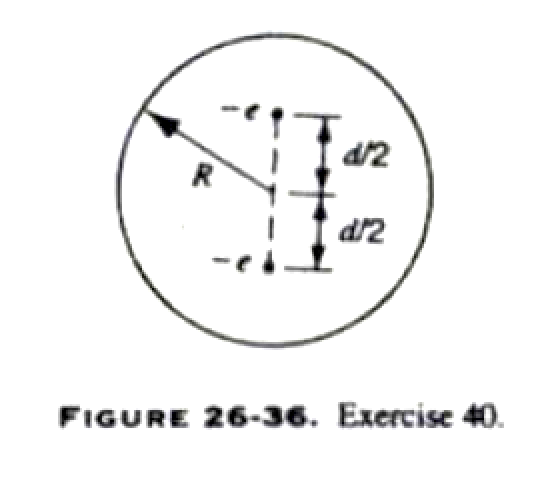
\includegraphics[scale=0.55]{26-36.png}
		\end{center}
		
	\end{problem}
	
	\begin{solution}
		\vfill
	\end{solution}
	\newpage
	
	
	
\end{document}